\documentclass{brochure}
\usepackage{lipsum}

\renewcommand\docType{Document Type (define docType)}
\renewcommand\productName{Product (productName)}
\renewcommand\email{dummy@eatabattery.com}
\renewcommand\phone{(111) 222-3333}
\renewcommand\website{eatabattery.com}
\renewcommand\company{Eat A Battery LTD.}

\renewcommand\addressA{123 Duracell Ave, 9V}
\renewcommand\addressB{Scranton, PA 12345}
\renewcommand\logo{logo.pdf}

\begin{document}

%\iffalse
\begin{brochure}
\begin{page}

\sectionTitle{Section}
\lipsum[25]

\sectionTitle{Section2}
\lipsum[55]
		\begingroup
		\begin{center}
				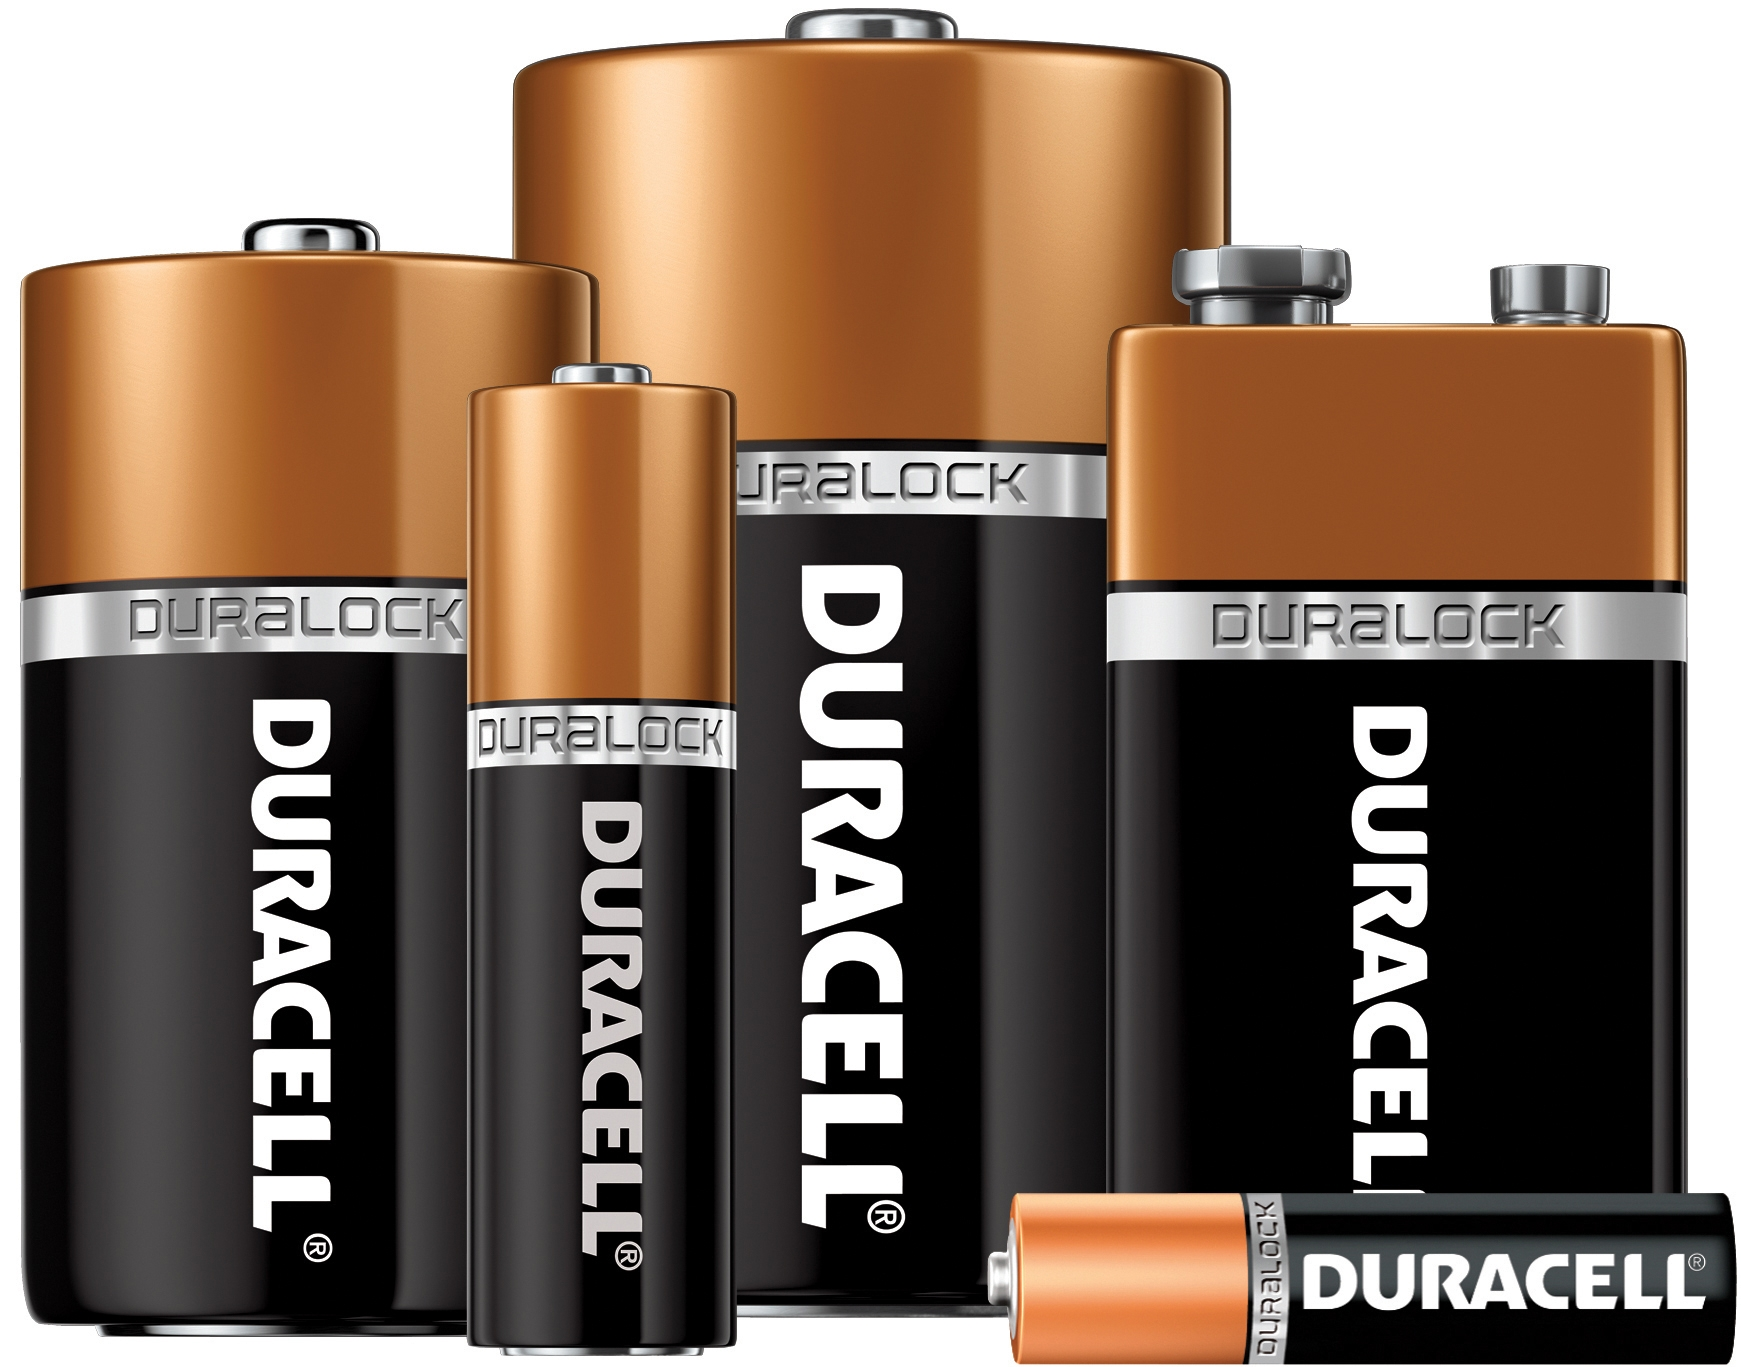
\includegraphics[width=.75\linewidth]{lunch}
				\captionof{figure}{capt}
				\end{center}
		\endgroup

\vspace{-11pt}
\lipsum[75]
		\vspace{11pt}
		\begin{infoBox}{Construction}
			\lipsum[8]
		\end{infoBox}

\end{page}


\begin{lastpage}
		\begingroup
				\begin{center}
				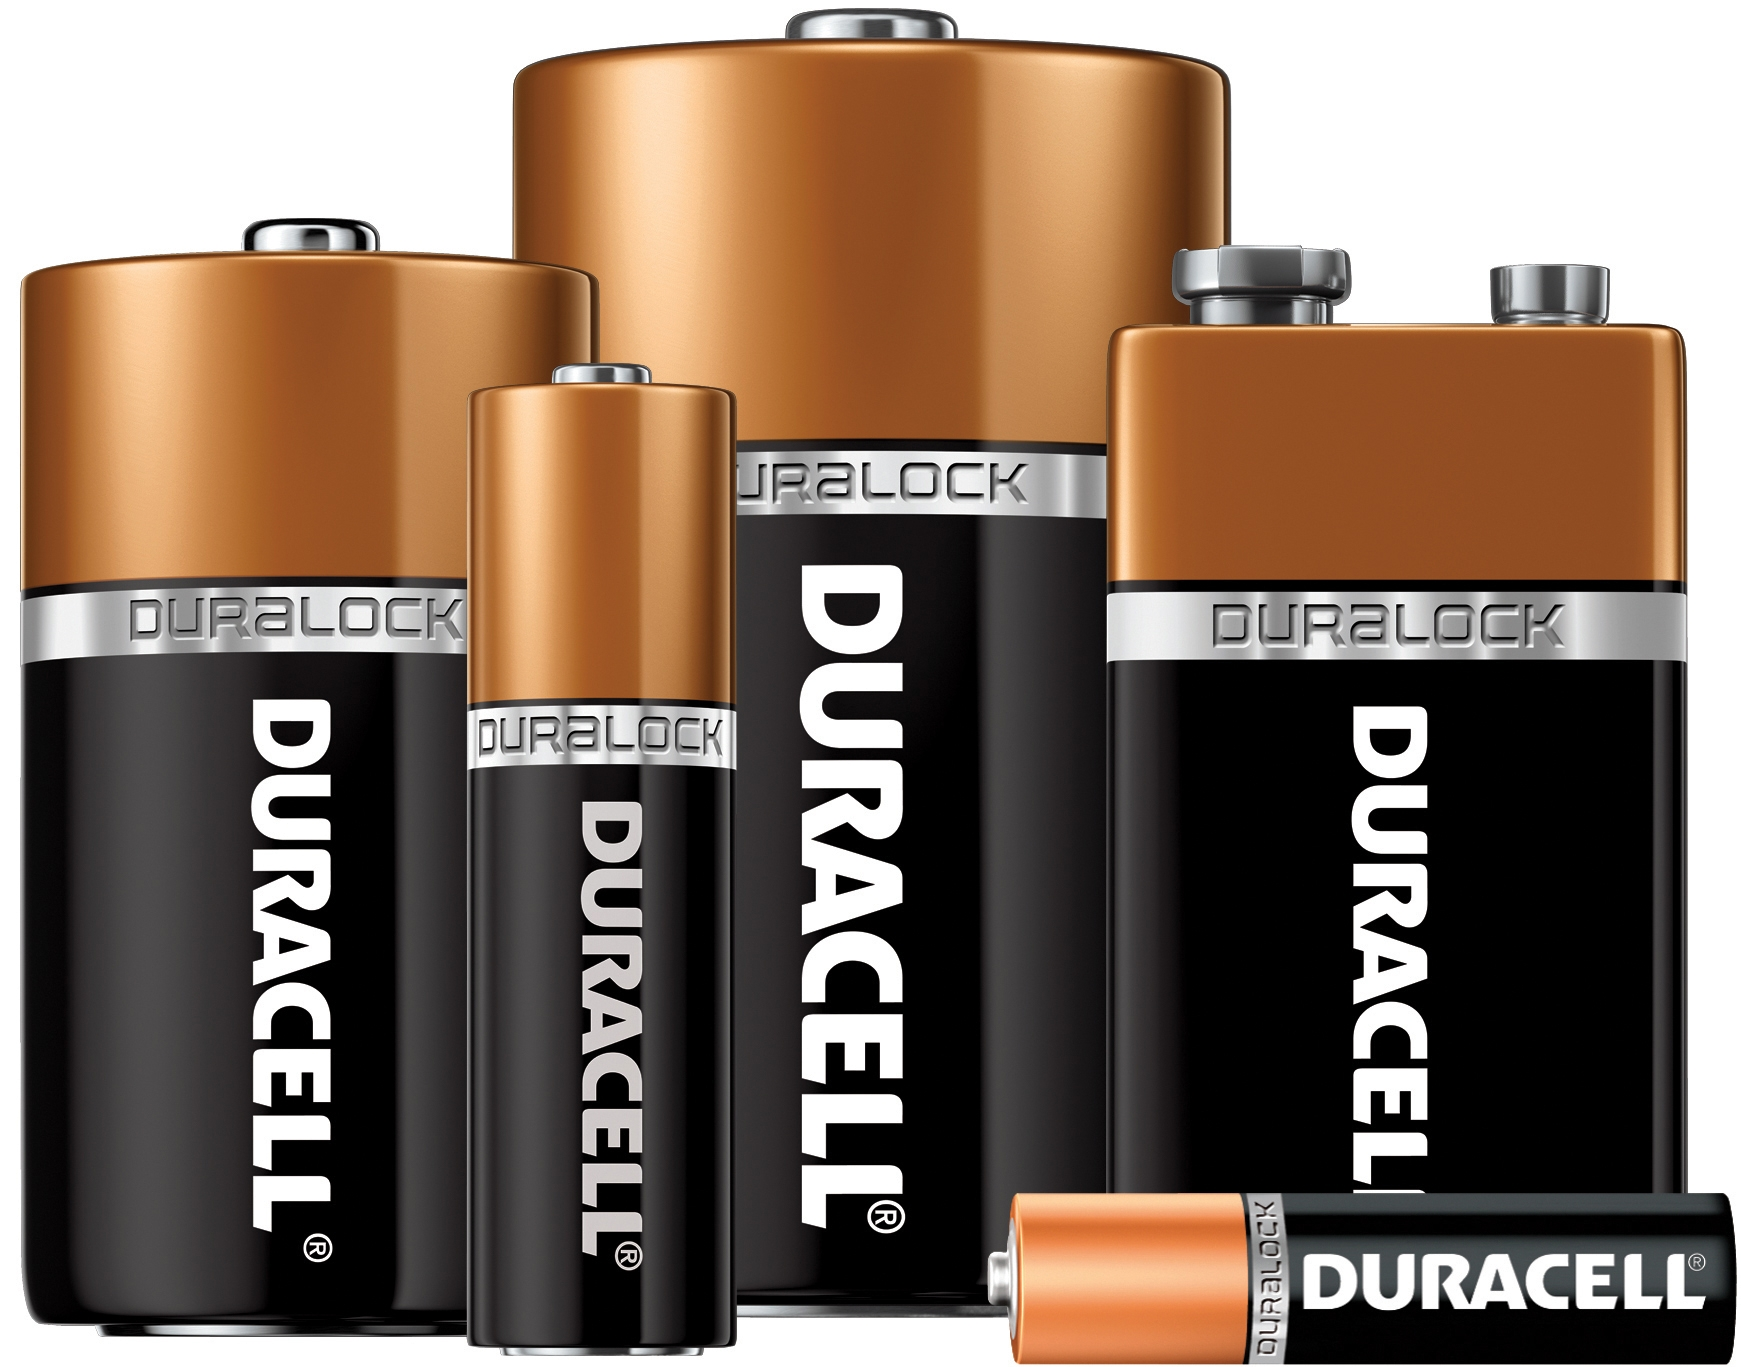
\includegraphics[width=\linewidth]{lunch}
				\captionof{figure}{\small Noise spectra of the QL01-B.
				It is shot-noise limited at $\geq$~7~nA
				(DC-100~kHz) and $\geq$~25~nA (DC-1~MHz).}
				\label{fig:noisePlot}
				\end{center}
		\endgroup
		\begin{infoBox}{Linearity}
			\lipsum[8]
		\end{infoBox}

		\begin{infoBox}{Spectral Response}
				\begin{modelCompare}
				\textbf{Spectral Response:} & See Figure \ref{fig:spectralResp} & See Figure \ref{fig:spectralResp}\\
				\textbf{Peak Response:} & 0.62 A/W& 0.65 A/W\\
				\textbf{Peak Wavelength:} & 850 nm & 870 nm\\
				\end{modelCompare}
		\end{infoBox}

		\begingroup
				\begin{center}
				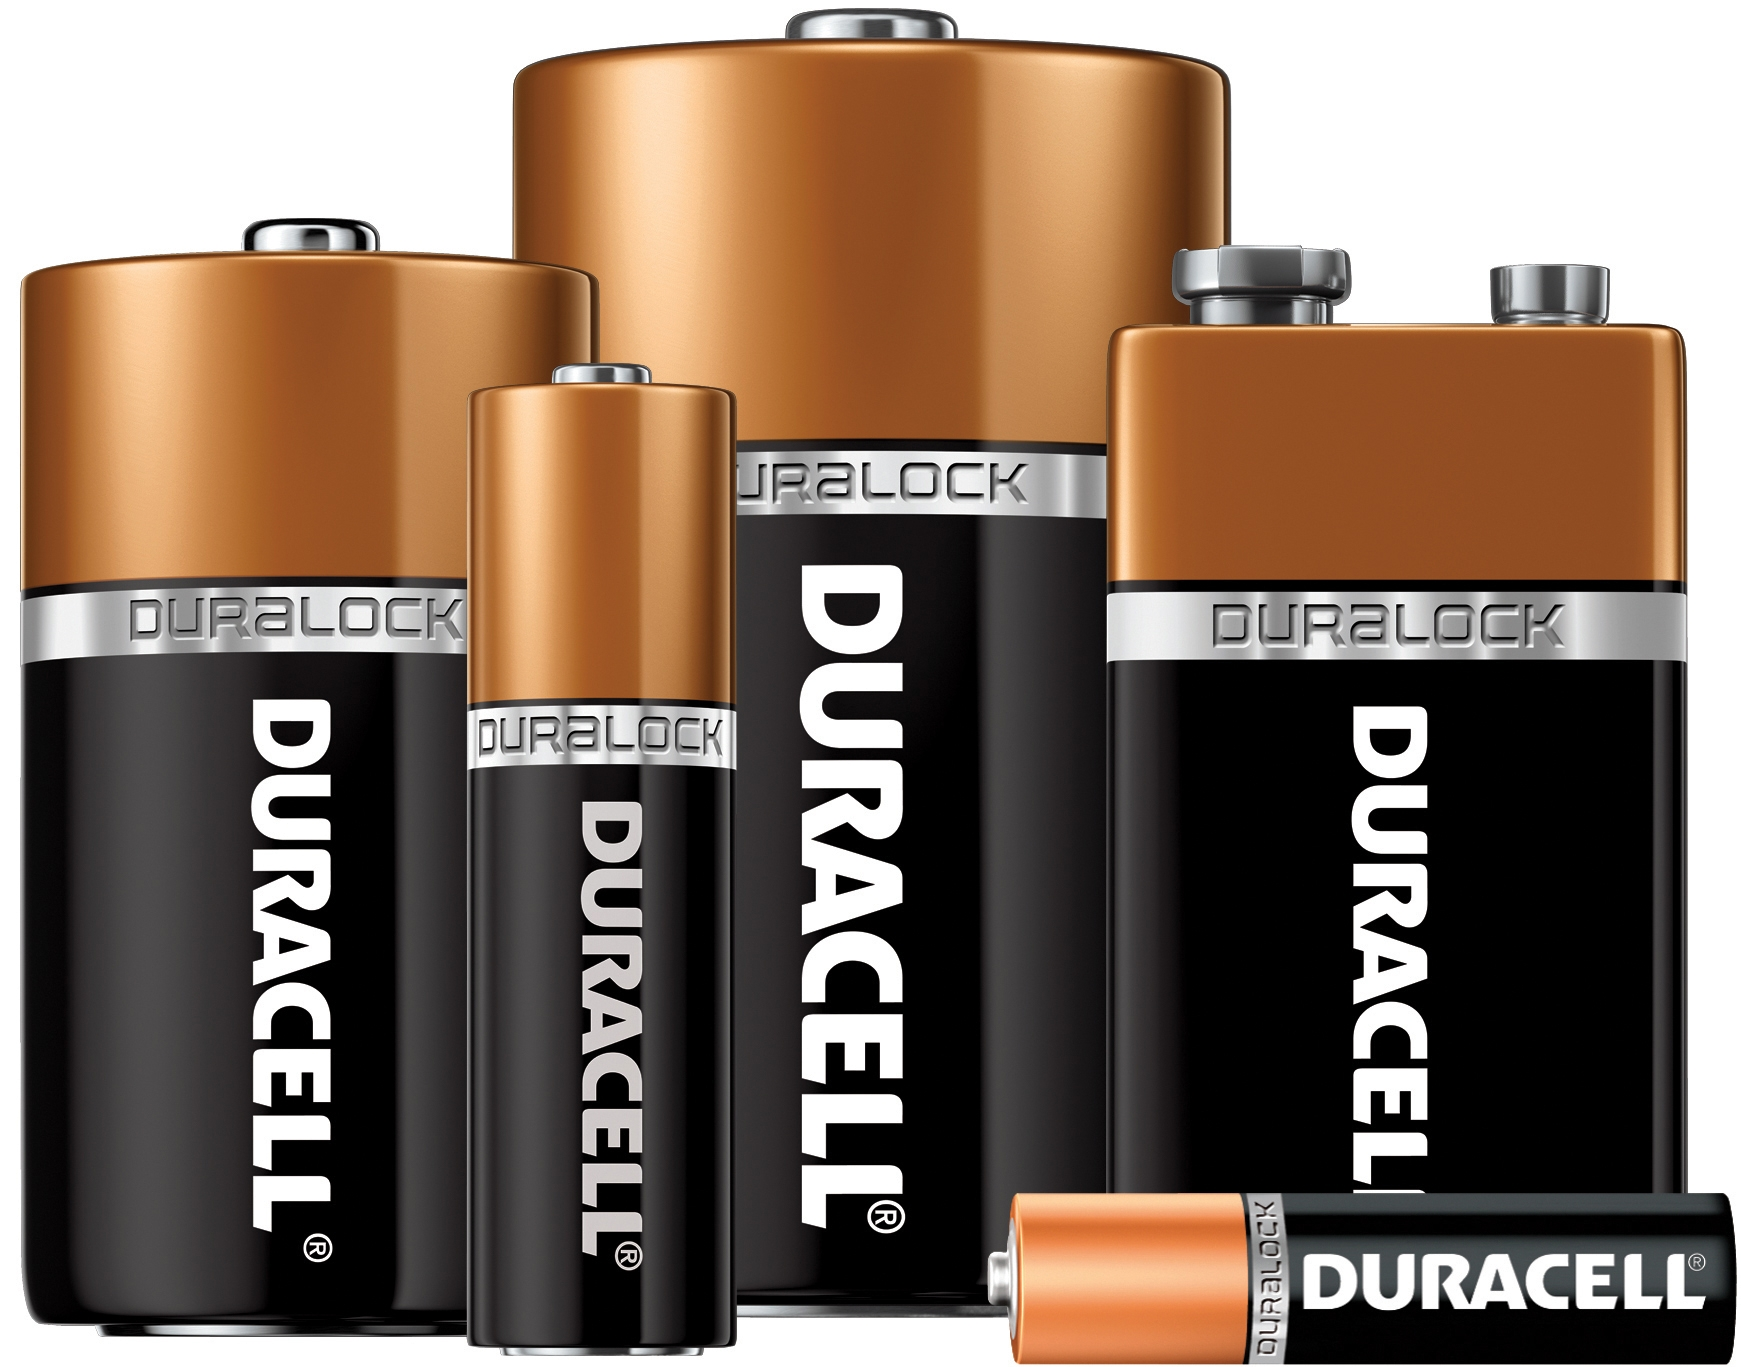
\includegraphics[width=\linewidth]{lunch}
				\captionof{figure}{\small Quantum efficiency of the
				QL01-A/B \emph{vs} wavelength, showing $>$ 90\%
				peak QE.}
				\label{fig:spectralResp}
				\end{center}
		\endgroup

		\grayLine{.5\linewidth}
		\begin{infoBox}{Resources}
		\begin{tabular}{l l}
		\textbf{Thing 1:} &\url{eatAbattery.com}\\
		\textbf{Thing 2:} &\url{eatAbattery.com}\\
		\textbf{Thing 3:} &\url{eatAbattery.com}\\
		\end{tabular}
		\end{infoBox}

		\end{lastpage}
\end{brochure}
%\fi
\end{document}
